\chapter{Métrica mixta}
Como vimos en el capitulo 4 existen diferentes algoritmos de reconocimiento de agrupamientos que pueden ser utilizados para detectar, con diferente grado de granularidad, grupos de genes coexpresados.\\\\
Dichos algoritmos reportan conjuntos de genes que muestran un nivel de correlación transcripcional alto, pero pueden diferir notablemente en el grado de coherencia biológica que es posible asociar a dichas estructuras.\\\\
En este capítulo utilizaremos los resultados obtenidos en el capítulo 6 para desarrollar un procedimiento que integre la información contenida en el espacio de expresión con la información contenida en el espacio de conocimientos GO, para favorecer la búsqueda de estructuras biológicamente coherentes. La idea principal es la de montar sobre la heterogeneidad topológica embebida en la estructura de aristas de la red inferida a partir de información transcripcional, un desorden adicional modificando el valor de los pesos de dichas aristas en función de la coherencia biológica local hallada en cada caso. De esta manera, pretendemos obtener una métrica mixta que contenga información de ambos espacios.

\section{Hacia una métrica mixta}
Existen muchas formas de mezclar las métricas del espacio de expresión y del espacio GO. Una de las métricas mixtas investigadas previamente por el grupo \cite{Berenstein2010} fue la de mezcla convexa de distancias, donde se define una nueva distancia $d_{mix}$ a partir de las distancias de expresión y GO y un parámetro $\alpha$ que controla la contribución de cada métrica al algoritmo:
\begin{equation}
	d_{mix} = \sqrt{\alpha d_{x}^2 + (1-\alpha)\tilde{d}_{GO}^2}
\end{equation}
con $\tilde{d}_{GO} = \frac{\langle d_x \rangle}{\langle d_{GO} \rangle}d{_GO}$, de tal manera que coincidan los valores medios de ambas distribuciones de distancia.\\\\
Esta métrica busca el consenso a partir del parámetro global $\alpha$, que parametriza de manera continua una métrica en contraposición con la otra.\\\\
Para este trabajo, implementamos una métrica mixta que en lugar de buscar el consenso entre las métricas, penaliza las correlaciones no soportadas por las distintas ontologías e incentiva aquellas que si lo están.
\subsection{Modulación de heterogeneidades transcripcionales con información biológica}
Partiendo de la red de 30 primeros vecinos mutuos, $30kmnn$, con información transcripcional contenida en los patrones de conectividad de la red, buscamos incluir información biológica en el esquema de conexionado de la misma. Para ello, modificaremos los pesos de las aristas utilizando la información de coherencia biológica presente en KTA, tomando cada tratamiento y calculando el KTA promedio de toda la red y el KTA local de cada arista. Estas dos cantidades, el KTA promedio, que llamaremos $KTA_{fondo}$, y el KTA local de la arista entre dos nodos $i$ y $j$, que llamaremos $KTAl_{ij}$, se relacionan en una cantidad que llamaremos $stress$ y que utilizaremos como criterio para identificar si debemos penalizar o incentivar una correlación en el espacio de expresión. El $stress$ se define como:
\begin{equation}
	stress = \frac{KTA_{fondo}}{KTAl_{ij}}
	\label{eq:stress}
\end{equation}
Si $KTAl_{ij} > KTA_{fondo}$, se obtiene un $stress < 1$, mientras que si $KTAl_{ij} < KTA_{fondo}$, obtenemos que $strees > 1$. Por lo tanto, si realizamos la transformación no lineal de la similaridad de correlación:
\begin{equation}
	w_{ij} = simcor_{ij}^{stress}
	\label{eq:pesos_de_la_red}
\end{equation}
obtenemos unos nuevos pesos para la similaridad en donde aquellas relaciones que son similares en GO ($KTAl_{ij} > KTA_{fondo}$) serán incentivadas en el espacio de expresión y a la inversa, las que no son similares en GO serán penalizadas en el espacio de expresión. Los valores típicos del $stress$ oscilan entre ($0.8$ y $1.2$). Si graficamos la distribución de fuerza o \textit{strength} para los nodos de la red con los pesos modificados, definida como:
\begin{equation}
	S_i = \sum_j w_{ij}
	\label{eq:strength}
\end{equation}
obtenemos la que se observa en la figura \ref{fig:distribucion_strength_beta_1}. Esta distribución es muy similar a la distribución de grado, $P(k)$, y esto es razonable, ya que los pesos $w_{ij}$ son muy cercanos a 1 debido a la alta correlación entre vecinos de un nodo y los valores típicos de $stress$. Para poder maximizar efectivamente la heterogeneidad a nivel de pesos con información biológica, buscaremos un parámetro $\beta$ al cual elevar los pesos $w_{ij}$ tal que la distribución de \textit{strength} de la red siga una distribución de tipo ley de potencias, como propone Horvath, en \cite{Horvath2005}.\\\\
\begin{figure}[t!]
    \centering
    \begin{subfigure}[t]{0.45\textwidth}
    \centering
    \includegraphics[width=1\textwidth]{distribucion_strength_beta_1.pdf}
    \caption{Logaritmo de la distribución de $strength$ para la red $30knmm$ con pesos $w_{ij}$ y $\beta=1$ del tratamiento 'Frío'.}
    \label{fig:distribucion_strength_beta_1}
    \end{subfigure}    
    \begin{subfigure}[t]{0.45\textwidth}
    \centering
    \includegraphics[width=1\textwidth]{distribucion_strength_beta_4.pdf}
    \caption{Logaritmo de la distribución de $strength$ para la red $30knmm$ con pesos $w_{ij}$ y $\beta=4$ del tratamiento 'Frío'. En rojo ajuste lineal (R cuadrado = 0.9).}
    \label{fig:distribucion_strength_beta_4}
    \end{subfigure}    
    \caption{Logaritmo de la distribución de $strength$ para la red $30knmm$ con pesos $w_{ij}$ y distintos $\beta$ del tratamiento 'Frío'.}
\end{figure}
Buscamos el parametro $\beta$ adecuado realizando un barrido para $\beta$ desde 1 hasta 4 con pasos de 1 y desde 15 hasta 65 con pasos de 5, transformando los pesos de la red como:
\begin{equation}
	w_{ij}^{'} = w_{ij}^{\beta}
	\label{eq:pesos_beta}
\end{equation}
y realizando luego un ajuste lineal para el logaritmo de la distribución de \textit{strength}. Tomamos el parámetro $\beta$ que mejor ajustaba cada tratamiento en el sentido de R cuadrado y lo utilizamos para modificar los pesos $w_{ij}$. Por ejemplo, para el tratamiento 'Frío', obtuvimos $\beta=4$ como muestra la figura \ref{fig:distribucion_strength_beta_4}.
\subsection{Heterogeneidades en escala de grupo}
La idea de nuestro enfoque es partir de los grupos detectados en el espacio transcripcional y estudiar como se comportan en términos de su coherencia biológica. Para ello pretendemos analizar heterogeneidades transcripcionales, en la escala interna al grupo, modificando la similaridad de correlación con la información obtenida mediante el índice KTA local en las redes de 30 primeros vecinos mutuos.\\\\
Para ello, tomamos cada grupo de cada tratamiento y calculamos el KTA de todo el grupo, además del KTA local de cada arista del grafo $30kmnn$ correspondiente al grupo. Con estas dos cantidades redefiniremos el $stress$ para que sea un $stress$ referido al grupo. La figura \ref{fig:distribucion_de_stress} presenta la distribución de $stress$ para el tratamiento 'Frío' en función del tamaño de grupo. Se observa que el $92\%$ de los valores de $stress$ se ubica entre $0.8$ y $1.2$, como habíamos mencionado previamente. 
\begin{center}
\includegraphics[width=0.8\textwidth]{distribucion_de_stress}
\captionof{figure}{Boxplot con la distribución de $stress$ para el tratamiento 'Frío' y ontología CC en función del tamaño de grupo.}
\label{fig:distribucion_de_stress}
\end{center}
Una vez obtenidos los parámetros para la métrica mixta, desarrollamos un método heurístico para poder aplicar esta nueva métrica mixta en el proceso de detección de agrupaciones de genes.

\section{Método heurístico}
El método heurístico desarrollado consiste en tomar cada grupo de una partición realizada previamente con corte de árbol dinámico e intentar encontrar subestructura dentro del mismo a partir de la métrica mixta arriba presentada de tres formas distintas.\\\\
La primera forma consiste en aplicar sobre cada grupo nuevamente un corte de árbol dinámico, utilizando la ahora métrica mixta en la confección del dendrograma, es decir: penalizando (incentivando) las conexiones más importantes, que son las que aparecen en la red de k primeros vecinos mutuas con alto (bajo) stress. A este método lo llamaremos \textit{lkta.dtc}. Por otro lado, la segunda y la tercera formas, que llamaremos \textit{lkta.infomap} y \textit{lkta.cnm}, consisten en obtener comunidades mediante infomap y cnm, respectivamente, en la red de los genes del grupo original, teniendo en cuenta los pesos modificados por la métrica mixta.\\\\
En todos los casos, una vez obtenida una partición del grupo, calculamos el índice BHI de los subgrupos obtenidos que no alcanzaron un nivel de significancia biológica suficiente y volvemos a unir aquellos subgrupos que se encuentren por debajo de una desviación estandar del control nulo 1 presentado en la sección \ref{subsec:control_nulo}. Esto lo hacemos mediante un algoritmo voraz o greedy, que en cada paso busca los dos subgrupos tales que el BHI de los dos juntos sea superior al BHI de cada uno por separado. Cuando el algoritmo no consigue unir dos subgrupos para mejorar el BHI, se detiene.\\\\ Finalmente, todos los subgrupos que todavía quedan por debajo de una desviación estandar del control nulo 1 son unidos entre sí en un único subgrupo.\\\\
Además de las 3 metodologías descriptas, utilizaremos un cuarto método, llamado \textit{insideX}, a modo de control. El mismo consiste en volver a particionar cada grupo usando corte de árbol dinámico con $deepsplit=4$, pero sin cambiar la métrica por la métrica mixta. Esto nos permitirá controlar la efectividad de la métrica mixta para encontrar mayor resolución en las particiones.\\\\
Para cuantificar el cambio en la información biológica que brinda la nueva partición, elegimos tomar el valor medio del BHI de los subgrupos, $\langle BHI \rangle$, y el valor medio del BHI de los subgrupos que superan el control nulo, $\langle BHI \rangle _{+}$. Esta ultima cantidad refleja la situación de aquellas subestructuras del grupo original que se ``beneficiaron'' desde el punto de vista del BHI, con la mayor granularidad de la nueva partición.\\\\
A modo de ejemplo, presentamos en las figuras \ref{fig:metodos_mixtos_grupo_2} y \ref{fig:metodos_mixtos_grupo_9} los resultados de esta heurística aplicada a los grupos 2 y 9 del tratamiento 'Frío'. En las mismas, la curva negra indica 1 $\sigma$, la roja 2 $\sigma$ y la verde 3 $\sigma$ de la distribución del BHI del control nulo 1. El punto lleno representa el grupo original y su BHI. En verde si su BHI supera el control nulo y en rojo si no. Los puntos vacíos en gris representan los subgrupos nuevos. En la leyenda, el primer número es $\langle BHI \rangle$ y el segundo, entre paréntesis, es $\langle BHI \rangle _{+}$.\\\\
\clearpage
\begin{sidewaysfigure}[H]
 \centering
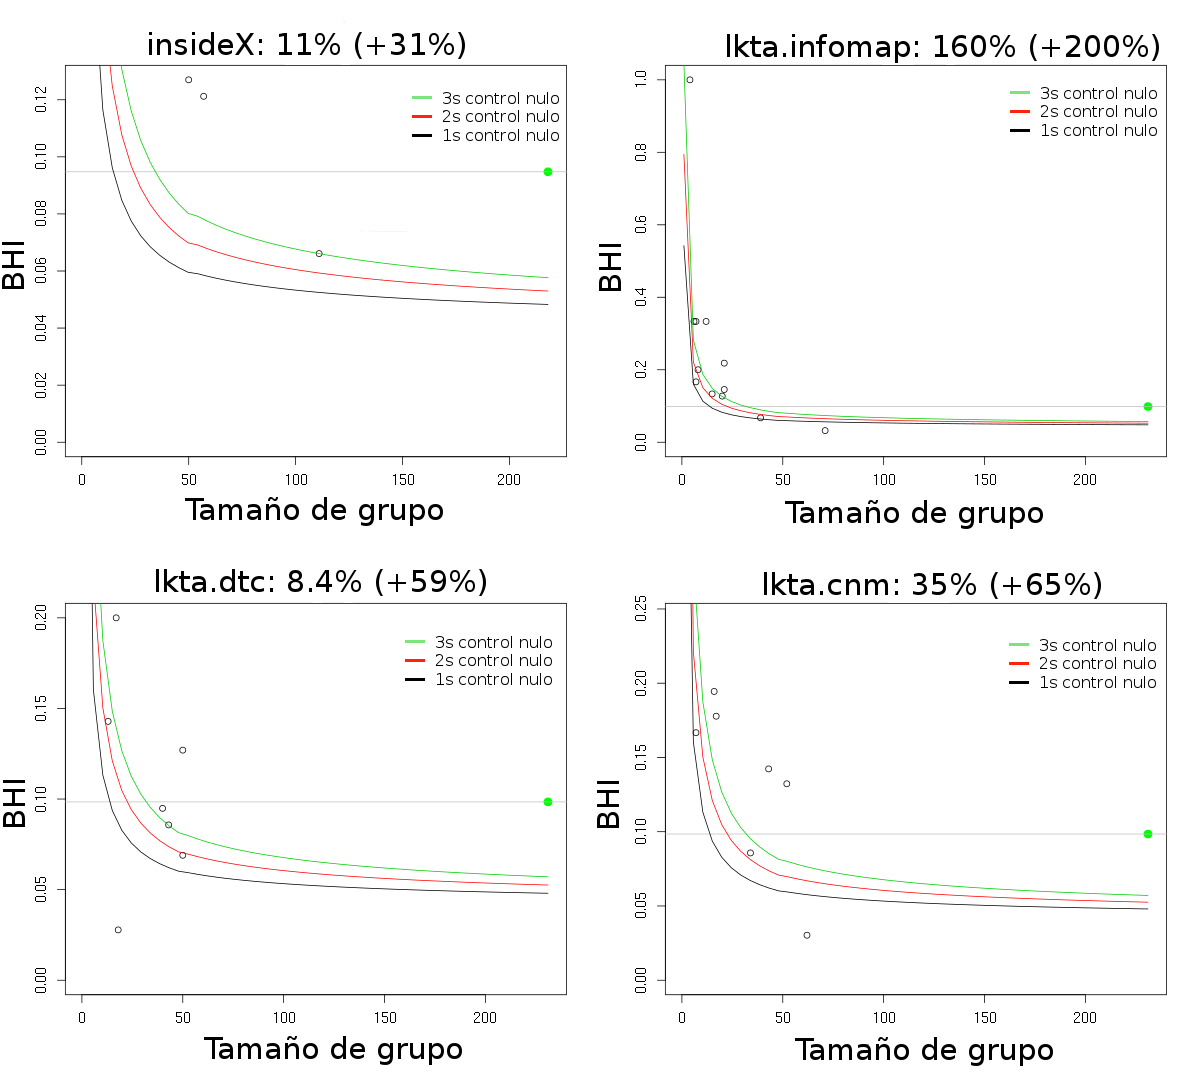
\includegraphics[width=0.7\textwidth]{metodos_mixtos_grupo_2}
\captionof{figure}{Métodos con métrica mixta y control para el grupo 2 del tratamiento 'Frío'. La curva negra indica 1 $\sigma$, la roja 2 $\sigma$ y la verde 3 $\sigma$ de la distribución del BHI del control nulo 1. El punto lleno representa el grupo original y su BHI. En verde si su BHI supera el control nulo y en rojo si no. Los puntos vacíos en gris representan los subgrupos nuevos. En la leyenda, el primer número es $\langle BHI \rangle$ y el segundo, entre paréntesis, es $\langle BHI \rangle _{+}$.}
\label{fig:metodos_mixtos_grupo_2}
\end{sidewaysfigure}

\begin{sidewaysfigure}[H]
 \centering
\includegraphics[width=0.7\textwidth]{metodos_mixtos_grupo_9}
\captionof{figure}{Métodos con métrica mixta y control para el grupo 9 del tratamiento 'Frío'. La curva negra indica 1 $\sigma$, la roja 2 $\sigma$ y la verde 3 $\sigma$ de la distribución del BHI del control nulo 1. El punto lleno representa el grupo original y su BHI. En verde si su BHI supera el control nulo y en rojo si no. Los puntos vacíos en gris representan los subgrupos nuevos. En la leyenda, el primer número es $\langle BHI \rangle$ y el segundo, entre paréntesis, es $\langle BHI \rangle _{+}$.}
\label{fig:metodos_mixtos_grupo_9}
\end{sidewaysfigure}

\clearpage
Se observa que para el grupo 2, un grupo con un BHI por sobre el control nulo y el segundo grupo más grande de la partición, el método \textit{insideX} logró encontrar heterogeneidades y partir el grupo, obteniendo tres subgrupos de más de 50 genes cada uno y una mejora del 11\% en $\langle BHI \rangle$, y una del 31\% para $\langle BHI \rangle _{+}$. Por otro lado, los tres métodos \textit{lkta} lograron superar la mejora obtenida por \textit{insideX} en $\langle BHI \rangle _{+}$, y tanto \textit{lkta.infomap} como \textit{lkta.cnm} lograron mejorar además el obtenido en $\langle BHI \rangle$, siendo \textit{lkta.infomap} el que mejores puntajes logró, llegando a obtener incluso un grupo con un BHI de $0.97$.\\\\
Para el grupo 9, un grupo con un BHI por debajo del control nulo y relativamente pequeño, el método \textit{insideX} no logró encontrar heterogeneidades dentro del grupo y por lo tanto no pudo particionarlo, sin lograr ningún tipo de mejora en el mismo. Sin embargo, todos los métodos \textit{lkta} lograron particionar el grupo y mejorar ambos índices, siendo nuevamente \textit{lkta.infomap} el que logró la mejora más significativa, con un 360\% de incremento en $\langle BHI \rangle$ y un 460\% de incremento en $\langle BHI \rangle _{+}$.\\\\
Finalmente, realizamos este análisis para todos los tratamientos y todos los grupos en cada tratamiento. Para cada método, graficamos el $\langle BHI \rangle$ de los subgrupos en función del BHI del grupo original en la figura \ref{fig:bhi_nuevo_vs_bhi_original}. En rojo, graficamos una recta de pendiente unitaria. Se observa que todos los métodos que utilizan la métrica mixta consiguieron grupos que no solo presentan altos valores de coherencia transcripcional sino que tienen BHI superiores a los que tenían originalmente. En particular, para lkta.infomap el 92\% de los grupos fue dividido en subgrupos que poseen un BHI promedio superior al de su grupo original, mientras que lo mismo sucede en un 91\% de los grupos para lkta.cnm y un 87\% para lkta.dtc. Finalmente, para el control insideX, solo el 10\% de los grupos mejoró su BHI promedio al ser particionado nuevamente.
\begin{center}
\includegraphics[width=0.8\textwidth]{bhi_nuevo_vs_bhi_original_p.pdf}
\captionof{figure}{BHI nuevo en función de BHI original para todos los tratamientos, todos los grupos y los cuatro métodos heurísticos. En rojo, una recta de pendiente unitaria.}
\label{fig:bhi_nuevo_vs_bhi_original}
\end{center}
\section{Interpretación biológica}
Una vez obtenidos los nuevos grupos mediante los distintos métodos, buscaremos ganar conocimiento sobre el significado biológico de cada grupo y en particular estudiaremos si los genes dentro de un mismo grupo participan de algún proceso biológico común. Para ello, recurriremos al análisis de sobreexpresión de conceptos GO dentro de un dado agrupamiento de genes.\\\\
El mismo consiste en considerar un grupo de genes y analizar si existen categorías de una ontología (BP u CC), sobrerepresentadas en el mismo, utilizando una prueba de Fisher exacta con un p-valor $<10e-4$.\\\\
Ilustraremos los resultados de esta tipo de análisis considerando los grupos 2, 6 y 13 del tratamiento 'Frío'. En la figura \ref{fig:metodos_mixtos_2_6_13} se observan los grupos originales y los subgrupos obtenidos por medio de cada método junto con el control nulo 1 y los correspondientes valores de BHI, mientras que en las figuras \ref{fig:fisher_grupo_2}, \ref{fig:fisher_grupo_6} y \ref{fig:fisher_grupo_13} se visualizan los resultados de la prueba exacta de Fisher para cada uno de estos grupos.
\clearpage
\begin{center}
\includegraphics[width=0.8\textwidth]{metodos_mixtos_2_6_13}
\captionof{figure}{En la primera, segunda y tercera columna se consignan los resultados del análisis para grupos transcripcionales 2, 6 y 13 del tratamiento 'Frío' respectivamente. La primer, 2da y 3era fila muestran los métodos dtc, cnm e infomap. El círculo verde representa el grupo original. Los cuadrados son subgrupos, con el nivel de grisado dependiente del alejamiento de las curvas de control. Las curvas punteadas son 1 $\sigma$, 2 $\sigma$ y 3 $\sigma$ de la distribución del BHI del control nulo 1.}
\label{fig:metodos_mixtos_2_6_13}
\end{center}
En el Panel izquierdo: mapa de colores o \textit{heatmap} de p-valores donde las filas representan categorías de la ontología GOBP, y las columnas subgrupos del grupo transcripcional 2 detectados por la metodología insideX y las 3 variantes lkta.\\\\
El color corresponde al nivel de significancia obtenido en el test de sobrerepresentacion.\\\\ 
Para una mejor interpretabilidad se utilizaron los 50 conceptos GO relevantes (sobrerepresentados) mas específicos y se ordenaron según un dendrograma generado a partir de la similaridad semántica de los mismos.\\\\
Se incluye en el panel central detalle sobre el contenido de información, el nivel de profundidad en la jerarquía de la ontología y la descripción de los conceptos GO respectivos.\\\\
En el panel derecho: conceptos GO de menor especificidad para mejorar la interpretabilidad.

\begin{sidewaysfigure}[H]
 \centering
\includegraphics[width=0.9\textwidth]{fisher_grupo_2_p}
\captionof{figure}{Resultado del test de sobreexpresión de nodos GO para el grupo 2 del tratamiento 'Frío' para los métodos con métrica mixta y control.}
\label{fig:fisher_grupo_2}
\end{sidewaysfigure}

\begin{sidewaysfigure}[H]
 \centering
\includegraphics[width=0.9\textwidth]{fisher_grupo_6_p}
\captionof{figure}{Resultado del test de sobreexpresión de nodos GO para el grupo 6 del tratamiento 'Frío' para los métodos con métrica mixta y control.}
\label{fig:fisher_grupo_6}
\end{sidewaysfigure}

\begin{sidewaysfigure}[H]
 \centering
\includegraphics[width=0.9\textwidth]{fisher_grupo_13_p}
\captionof{figure}{Resultado del test de sobreexpresión de nodos GO para el grupo 13 del tratamiento 'Frío' para los métodos con métrica mixta y control.}
\label{fig:fisher_grupo_13}
\end{sidewaysfigure}

Para el grupo 2, el segundo grupo más grande de la partición, de 231 genes, y el método insideX, se observa que uno de los dos subgrupos con ganancia en BHI, el de 50 genes, explica casi en su totalidad los procesos biológicos del grupo original, mientras que no se encontró en el otro subgrupo con ganancia nodos sobreexpresados. Por otro lado, para lkta.dtc y lkta.cnmse se obtuvo un subgrupo de 50 genes con ganancia en BHI que explica los procesos del grupo original mientras que el resto de los subgrupos con ganancia no realiza aportes significativos al conocimiento biológico. Finalmente, para lkta.infomap, el de mayor ganancia en el índice BHI, ninguno de los subgrupos logra explicar los nodos sobreexpresados.\\\\
Pareciera que dentro del grupo transcripcional original (231 genes) un subgrupo de 50, detectado por 2 de las variantes lkta y la puramente transcripcional (insideX), es el responsable del enriquecimiento. El hecho de que insideX lo haya detectado sugiere que aun heterogeneidades puramente transcripcionales, puestas de manifiesto en la escala del grupo 2, correlacionan con la congruencia biológica del subgrupo.\\\\
Es interesante notar que en este caso la alta granularidad de la partición infomap parece excesiva en términos de intepretación biológica.\\\\
Para el grupo 6, un grupo de tamaño intermedio, con 149 genes, el método insideX consigue nuevamente dos subgrupos con ganancia en BHI, de 59 y 52 genes respectivamente, que explican en conjunto la mayor parte de los nodos sobreexpresados del grupo original. Para lkta.dtc se obtienen dos subgrupos informativos de tamaño pequeño, de 18 y 17 genes respectivamente. Para lkta.cnm y lkta.infomap se obtuvieron un subgrupo informativo de 49 y otro de 26 genes respectivamente.\\\\
En este caso los 3 métodos lkta detectan estructuras que se pueden asociar a los mismos conceptos biológicos.\\\\
La resolución de la partición insideX parece detectar estructuras mas grandes, pero aun permite identificar conceptos biológicos similares en relación a los subgrupos encontrados.\\\\
Finalmente, para el grupo 13, un grupo pequeño de 41 genes, el método insideX no logró producir subgrupos, mientras que solo para lkta.cnm y lkta.infomap se consiguieron grupos explicativos para un grupo de 12 y otro de 10 genes respectivamente.\\\\
En este caso, solo el uso de la metodología lkta pudo detectar subestructura relevante. Cabe notar que se trata de conjuntos muy chicos de genes, por lo que es de esperar una mayor divergencia entre la estimación de congruencia biológica dada a partir de significancia de test de sobrerepresentacion y la asociada al índice BHI (que solo exige coincidencia en un grupo, sin importar su especificidad).\\\\
En lineas generales, observamos que en varios casos una gran parte de los nodos sobreexpresados del grupo original podían ser explicados por uno o dos subgrupos de tamaño reducido, lo que implica que existen efectivamente heterogeneidades en los grupos originales que no podía detectar el método de agrupamiento inicial $ds1$. Por otro lado, las estructuras detectadas fueron de tamaños intermedios, de alrededor de 50 o 60 genes. Esto da un indicio de que esta podría ser la resolución o escala a la cual deberíamos trabajar con los métodos de agrupamiento. Finalmente, este análisis nos permite ver que si bien lkta.infomap genera las particiones de grupos con mayor ganancia en el índice BHI, los subgrupos obtenidos no necesariamente brindan información biológica. Esto podría deberse al tamaño tan reducido de los subgrupos, que no facilita su interpretación en términos de GO.




